\chapter{Polarised Inclusive and Semi-inlcusive Deeply-Inelastic Scattering}
\chaptermark{Polarised DIS and SIDIS}
\label{ch:2}

This chapter is devoted to the discussion of the two physical processes that are taken into account in this Thesis, that is inclusive and semi-inclusive DIS. In Sec.~\ref{sec:theo_fram} I present the theoretical framework necessary to describe DIS experiments, providing an expression for the cross-section of polarized DIS in terms of polarized structure functions. The phenomenological relations between structure functions and measured observables is briefly reviewed in Sec.~\ref{sec:phenom_DIS}. Then, in Sec.~\ref{subsec:PM_hadronic_tensor} I will derive the expectations for the structure functions in the context of PM, and in Sec.~\ref{sec:field_theoretic} I show how QCD affects these predictions. Finally, in Sec.~\ref{sec:SIDIS} I present the theoretical structure necessary for the description of SIDIS processes.

%___________________________________________________________________________
\section{Theoretical framework}
\label{sec:theo_fram}

Let us consider the inclusive inelastic scattering of a polarised lepton beam off a polarised nucleon
%%
\begin{equation}
    \ell(k,s) + N(P, S) \longrightarrow \ell'(k',s') + X(P_X) \,,
    \label{eq:DIS}
\end{equation}
%%
where $P$ is the four-momentum of the nucleon target and $k,k'$ are the four-momenta of the incoming ($\ell$) and outgoing $(\ell')$ leptons, respectively. The additional labels $S,s$ and $s'$ indicate the spin along the quantization direction of the target, the incoming and the outgoing leptons. Finally, $X$ indicates the sum of all undetected final states with collective momentum $P_X$. In the limit of large momentum transfer, this process is referred to as Deep Inelastic Scattering (DIS). In this Thesis, I will assume that the scattering is dominated by processes with only one photon exchanged, since the ranges of values in $Q^2$, provided by the present polarised data, never probe the region in which weak corrections become important\footnote{QCD corrections are henceforth neglected.}. The Feynman diagram of this process is shown in Fig.~\ref{fig:DIS_Feynamn}.
%%
\begin{figure}[t]
  \centering
  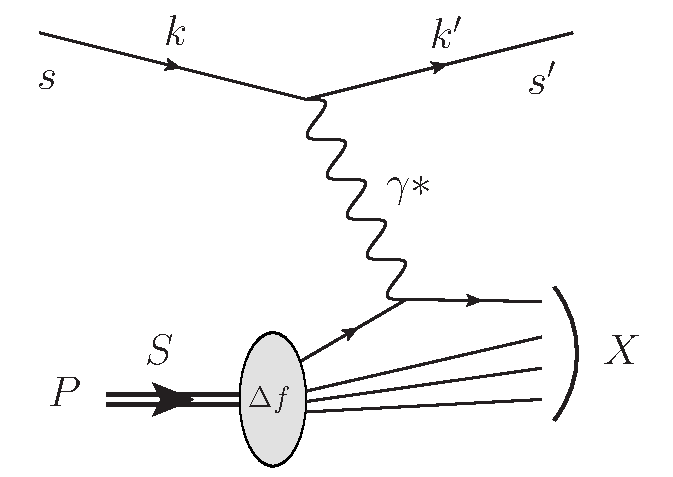
\includegraphics[width=0.5\textwidth]{DIS.pdf} 
  \caption{Feynman diagram for deep inelastic lepton-hadron scattering.}
  \label{fig:DIS_Feynamn}
\end{figure}
%%
The kinematics is worked out in the laboratory (LAB) reference frame, which corresponds to the fixed-target (FT) frame in polarised experiments\footnote{\footnotesize It must be observed that no polarised DIS experiments at colliders exist so far. Hence, in the polarised case the description can be limited to fixed-target experiments.}. The four-momenta are defined as follows
%%
\begin{equation}
    \begin{split}
        &k^{\mu} \;=\; \left(E, \vb{k} \right), \\
        &k'^{\mu} \;=\; \left(E', \vb{k'} \right), \\
        &P^{\mu} \;=\; \left(M, \vb{0} \right),
    \end{split}
\end{equation}
%%
where $M$ is the nucleon mass. I will make use of the following invariant variables
%%
\begin{align}
        & \nu = \frac{q \cdot P}{M} = E - E' \;\; \textrm{the energy lost by incoming lepton},
        \label{eq:nu}\\[5pt]
        & Q^2 = - q^2 \;\; \textrm{the virtuality of the exchanged photon},
        \label{eq:Q2}\\
        & x=\frac{Q^2}{2M\nu} \;\; \textrm{the Bjorken variable},
        \label{eq:x}\\
        & y = \frac{q\cdot P}{k \cdot P} = \frac{\nu}{E} \; \; \textrm{the energy fraction lost by the incoming lepton},
        \label{eq:y}\\
        & W^2 = \qty(P + q)^2 = M^2 + Q^2 \frac{1-x}{x} \;\; \textrm{the invariant mass of the system X}.
        \label{eq:W2}
\end{align}
%%
The process  is said to be "deep" when $Q^2 \gg M^2$ (\textit{i.e.} large momentum transfer), whereas the attribute "inelastic" is appropriate when $W^2 \gg M^2$ (\textit{i.e.} the hadron target is much inelastically excited). The amplitude for a process representing Fig.~\ref{fig:DIS_Feynamn}, with a generic final state $X$, is given by
%%
\begin{equation}
    \mathcal{M} = (-i e) \, \overline{u}(k',s') \, \gamma^{\mu}\, u(k,s) \, \frac{-i}{q^2} \, (-i e)\bra{X} j_{\mu}^{em} \qty(0) \ket{P,S} \,.
    \label{eq:ch2:amplitude}
\end{equation}
%%
Being a totally-inclusive process, no particular particles in the final state are detected. Hence, the total cross-section must take into account all the possible out-states, that is a sum over all the possible states $X$. For this reason, only two kinematic variables, among those listed in Eqs.~(\ref{eq:nu}-\ref{eq:W2}) are required to provide a complete description of the process. The differential cross-section for the process $2 \rightarrow 1 + n_X$ in the FT frame is given by 
%%
\begin{equation}
    d\sigma = \frac{1}{4 \qty|\vb{k}| M} \sum_{X} \qty| \mathcal{M} \qty( \ell N \rightarrow \ell'X ) |^2 \, \widetilde{d k'} \,  d\Phi_X \, ,
    \label{eq:ch2:dsigma}
\end{equation}
%%
where
%%
\begin{equation}
        d \Phi_X = \qty(2\pi)^4 \delta^{(4)} \qty( k + P - k' - P_X ) \widetilde{dP_X}  
\end{equation}
%%
and $\widetilde{dP_X}$ is the Lorentz invariant phase-space measure
%%
\begin{equation}
    \widetilde{d\, P_X} = \frac{d^3 \, P_X}{2 E_X (2\pi)^3} \,.
\end{equation}
%%
An identical definition holds also for $\widetilde{d k'}$.  Since the measurements in inclusive DIS concern only the final lepton $\ell'$, one can integrate over the entire momentum space in the hadron state and thus rewrite eq. \eqref{eq:ch2:dsigma} as
%%
\begin{equation}
    \begin{split}
        d\sigma &= \frac{1}{4 \qty|\vb{k}| M} \sum_{X} \int d\Phi_X \qty| \mathcal{M} \qty( \ell N \rightarrow \ell'X ) |^2 \widetilde{d k'}  \\
        & = \frac{1}{4 \qty|\vb{k}| M}  \frac{e^4}{q^4} \qty[ \overline{u}_{s'}(k') \, \gamma^{\mu}\, u_s(k)] \qty[\overline{u}_{s}(k) \,\gamma^{\nu}\, u_{s'}(k') ] \; \frac{d^3 \, k'}{2 E' (2\pi)^3} \times \\
        & \hspace{10mm} \sum_{X} \int d\Phi_X  \bra{X} j_{\mu}^{em} \qty(0) \ket{P,S} \; \bra{P,S} j_{\nu}^{em} \qty(0) \ket{X}  \\
        & = \frac{\alpha_{\textrm{em}}^2}{2 M \qty|\vb{k}| q^4} L_{\mu\nu} W^{\mu\nu} \qty|\vb{k}'| dE' d\Omega \,,
        \label{eq:ch2:dsigma2}
    \end{split}
\end{equation}
%%
where in the last equality I used $d^3 \, k' = \qty| \vb{k}' |^2 d|\vb{k}'| d\Omega$, and $d\Omega$ is the solid angle of the outgoing lepton in the LAB reference frame. The tensors $L_{\mu\nu}$ and $W_{\mu\nu}$ are defined as follows
%%
\begin{align}
    &L_{\mu\nu} = \qty[ \overline{u}_{s'}(k') \, \gamma^{\mu}\, u_s(k)] \qty[\overline{u}_{s}(k) \,\gamma^{\nu}\, u_{s'}(k') ] \,,
    \label{eq:ch2:lep_tens} \\
    &W_{\mu\nu} = \frac{1}{2\pi} \sumint_{X}  d\Phi_X  \bra{X} j_{\mu}^{em} (0) \ket{P,S}  \bra{P,S} j_{\nu}^{\dag em} (0) \ket{X}  \,,
    \label{eq:ch2:had_tens}
\end{align}
%%
where $\sumint_{X}$ is a shorthand notation to express the sum and the integral over the final state $X$. In the DIS limit, one can make use of the following approximations
%%
\begin{align}
    &k^2 = k'^2 \approx 0 \hspace{2mm} \Rightarrow \hspace{2mm} E \approx \qty| \vb{k} |, \hspace{2mm} E' \approx \qty| \vb{k'}|  \,,
    \label{eq:ch2:lep_approx}\\
    &Q^2 = - \qty(k - k')^2 \approx  2EE' \qty(1 - \cos \theta) = 4EE' \sin^2 \qty(\frac{\theta}{2}) \,,
    \label{eq:ch2:Q2_approx}
\end{align}
%%
where $\theta$ is the angle between the incoming and the scattered leptons. Inserting Eqs.~(\ref{eq:ch2:lep_approx},\ref{eq:ch2:Q2_approx}) in Eq.~\eqref{eq:ch2:dsigma2} one obtains 
%%
\begin{equation}
    \frac{d^2\,\sigma}{dE' \, d\Omega} = \frac{\alpha_{\textrm{em}}^2}{2MQ^4} \frac{E'}{E} L_{\mu\nu}W^{\mu\nu} = \frac{\alpha_{\textrm{em}}^2 E'}{s\, Q^4} L_{\mu\nu}W^{\mu\nu}\,,
    \label{eq:ch2:dsigma3}
\end{equation}
%%
where $s = (k + P)^2 \approx 2 M E$ is the Mandelstam variable. This expression gives the differential cross-section as a function of the energy of the outgoing lepton $E'$ and the scattered solid angle $\Omega$, both evaluated in the FT frame. It is possible to express Eq.~\eqref{eq:ch2:dsigma3} in terms of the Lorentz invariant dimensionless variables Eqs.~[\ref{eq:x}-\ref{eq:y}] by performing the transformation $(E', \theta) \rightarrow (x,y)$, which leads to
%%
\begin{equation}
    \frac{d^3 \, \sigma}{dx \, dy \, d\varphi} = \frac{\alpha_{\textrm{em}}^2 y}{2 Q^4} L_{\mu\nu} W^{\mu\nu} \,,
    \label{eq:ch2:dsigma4}
\end{equation}
%%
where $\varphi$ is the azimuthal angle of the scatted lepton. It is worth noting that, in computing Eq.~\eqref{eq:ch2:dsigma4}, the sum over the lepton and the hadron spin has not been taken into account. In principle, the lepton and hadron tensors can contain both symmetric and antisymmetric contributions. However, in the polarised case only the antisymmetric component survives, as I will show later.

%___________________________________________________________________________
\subsection*{Leptonic tensor}
The matrix element described by the lepton tensor can be decomposed into a symmetric and an antisymmetric part under $\mu \leftrightarrow \nu$ exchange. First, let us observe that the polarised spinor $u \qty(k, \, s)$, with polarisation vector $s$, satisfies the identity 
%%
\begin{equation}
    u \qty(k, \, s) \overline{u} \qty(k,\,s) = \frac{1}{2} (1 - \gamma_5 \slashed{s})  \qty(\slashed{p} + m)\,.
\end{equation}
%%
After summing over the spin of the scattered lepton $s'$, the lepton tensor can be written as a trace over gamma matrices
%%
\begin{equation}
    \begin{split}
        L_{\mu \nu} \qty(k,\,s;\, k') &= \frac{1}{2} \Trace \qty[ \qty(\slashed{k}' + m) \gamma_{\mu} \qty(1 - \gamma_5 \slashed{s}) \qty(\slashed{k} + m) \gamma_{\nu} ]\\
        & = \frac{1}{2} \Bigl\{ \Trace \qty[ \slashed{k} \gamma_{\mu} \slashed{k'} \gamma_{\nu} ] + m_{\ell} s^{\lambda} \Trace \qty[ \gamma_{\lambda} \gamma_{\nu} \gamma_{\rho} \gamma_{\mu} \gamma_{5} ] \qty( k - k' )^{\rho} \Bigr\}\\
        & = L_{\mu \nu}^{(S)} + i L_{\mu \nu}^{(A)} \,,
    \end{split}
\end{equation}
%%
where $L_{\mu \nu}^{(S)}$ and $L_{\mu \nu}^{(A)}$ are the symmetric and antisymmetric parts defined as 
%%
\begin{equation}
  L_{\mu \nu}^{(S)} \qty(k;\, k') = \frac{1}{2} \Trace \qty[ \slashed{k} \gamma_{\mu} \slashed{k'} \gamma_{\nu} ] = 2 \Bigl[k'_{\mu} k_{\nu} + k_{\mu} k_{\nu}' - g_{\mu \nu} \qty( k \cdot k' ) \Bigr]
\end{equation}
%%
\begin{equation}
  L_{\mu \nu}^{(A)} \qty(k,\,s;\, k') = \frac{1}{2i} m_{\ell} s^{\lambda} \Trace \qty[  \gamma_{\mu} \gamma_{\nu} \gamma_{\lambda} \gamma_{\rho} \gamma_{5} ] \qty( k - k' )^{\rho} = 2m_{\ell} \epsilon_{\mu \nu \lambda \rho } s^{\lambda} \qty( k - k' )^{\rho}\,.
\end{equation}
%%
If the momentum of the incoming lepton is aligned with the quantization axis, the spin vector can expressed as
%%
\begin{equation}
    s^{\mu} = \frac{\lambda_{\ell}}{m_{\ell}} k^{\mu}\, ,
    \label{eq:ch2:spin_vector}
\end{equation}
%%
where $\lambda_{\ell}$ is the helicity of the particle. It expresses whether the spin is parallel ($\lambda_{\ell} = +1/2$) or antiparallel ($\lambda_{\ell} = -1/2$) to the direction of motion of the particle. Thus, the antisymmetric component of the leptonic tensor can be finally expressed as
%%
\begin{equation}
    L_{\mu \nu}^{(A)} \qty(k,\,s;\, k') = 2\lambda_{\ell} \epsilon_{\mu \nu \lambda \rho} k^{\lambda} q^{\rho} \,,
    \label{eq:lep_tens_anti}
\end{equation}
%%
where the mass term $m_{\ell}$ has been cancelled by the denominator of Eq.~\eqref{eq:ch2:spin_vector}.

%________________________________
\subsection*{Hadronic tensor}
The hadronic tensor $W^{\mu \nu}$ encodes information on the proton structure. It receives non-perturbative contributions and, for that reason, its analysis cannot be addressed by a fully perturbative approach in QCD. However, exploiting symmetry constraints, the tensor can be decomposed into four scalar structure functions: the unpolarised functions $F_{1,2}$ and the helicity-dependent functions $g_{1,2}$, as long as parity violation is not concerned. Usually, these functions are measured by experiments and compared with theoretical predictions. These strongly depend on the theoretical model adopted to compute the observable, as I will show.%

In order to exploit symmetry constraints, I first rewrite the hadronic tensor as follows
%%
\begin{equation}
    \begin{split}
        W_{\mu\nu} &= \frac{1}{2\pi} \sumint_{\;\;X} \tilde{d P_X} \int d^4z \, e^{iz \cdot \qty(q + P - P_{X})}\bra{X} j_{\nu}(0) \ket{P,S} \bra{P,S} j^{\dag}_{\mu}(0) \ket{X}\\
        & = \frac{1}{2\pi} \sumint_{\;\;X} \tilde{d P_X} \int d^4z \, e^{iz \cdot q}\bra{X} j_{\nu}(0) \ket{P,S} \bra{P,S} j^{\dag}_{\mu}(z) \ket{X} \\
        & = \frac{1}{2\pi} \int d^4z \, e^{i z \cdot q} \bra{P,S} j^{\dag}_{\mu}(z) j_{\mu}(0) \ket{P,S} \,.
    \end{split}
    \label{eq:ch2:hadronic_tensor}
\end{equation}
%%
In the first line of Eq.~\eqref{eq:ch2:hadronic_tensor} the momentum-conservation delta function is expressed in its integral representation, introducing the dummy-variable z. The second line is the result of the transformation of the current-operator $j^{\dag}_{\mu}(0)$ by a space-time transformation 
%%
\begin{equation}
    \bra{P,S} j^{\dag}_{\mu}(0) \ket{X} =  \bra{P,S} e^{-i\hat{P}z} \, j^{\dag}_{\mu}(z) \, e^{i\hat{P}z} \ket{X} =  e^{-i z \cdot \qty(P - P_X )}\bra{P,S} j^{\dag}_{\mu}(z) \ket{X}\,.
\end{equation}
%%
Finally, the last line follows from the closure relation $\sumint_{\;\; X} \ket*{X} \bra*{X} = 1 $. In sanalogy with the lepton case, the hadronic tensor can be decomposed into a symmetric and an antisymmetric part
%%
\begin{equation}
    W_{\mu \nu} =  W_{\mu \nu} (q, \;P ) + i W_{\mu \nu} (q, \;P ; \; S ) \,.
\end{equation}
%%
Then, one can make the following observations:
\begin{enumerate}
    \item The hadronic tensor can be at most a function of $q, P$ and the spin vector of nucleon $S$, that is $W_{\mu \nu} = W_{\mu \nu}\qty(q,P;S)$.  
    \item The electromagnetic current must be conserved, that is $\partial \cdot j = 0$. In Eq.~\eqref{eq:ch2:hadronic_tensor}, this corresponds to the constraint $q_{\mu} W^{\mu \nu} = 0$.
    \item The hadronic tensor is hermitian, \textit{i.e.} $W_{\mu \nu} = \qty(W_{\mu \nu})^{*}$, as can be easily seen from eq. \eqref{eq:ch2:had_tens}. 
    \item The antisymmetric part of the hadroninc tensor is expected to change under reverse of the nucleon polarisation, hence the antisymmetric part must be linear in the polarisation vector.
    \item The strong interaction is parity invariant.
\end{enumerate}
Exploiting these constraints one finally obtains the most general form of the hadronic tensor \cite{collins_2011}
%%
\begin{equation}
  \begin{split}
  W_{\mu \nu}^{(S)} & = 2\qty(-g_{\mu \nu} + \frac{q_{\mu} q_{\nu}}{q^2}) F_1 \qty(x, Q^2) \\
  & + \frac{2 F_2 \qty(x , Q^2) }{P \cdot q} \qty(P_{\mu} - q_{\mu} \frac{P \cdot q}{q^2}) \qty(P_{\nu} - q_{\nu} \frac{P \cdot q}{q^2})\,,
  \label{eq:ch2:had_tens_final_symm}
  \end{split}
\end{equation}
%%
\begin{equation}
  \begin{split}
    W_{\mu \nu}^{(A)}  =  \epsilon_{\mu \nu \alpha \beta} \frac{q^{\alpha}2 M}{P \cdot q} \Biggl\{S^{\beta} g_1 \qty(x, Q^2) + \qty(S^{\beta} - P^{\beta} \frac{S \cdot q}{P \cdot q}) g_2 \qty(x,Q^2) \Biggr\} \,,
    \label{eq:ch2:had_tens_final_anti}
  \end{split}
\end{equation}
%%
The spin-independent coefficients $F_1,\, F_2$ and the spin-dependent ones $g_1,\,g_2$ are usually called \textit{structure functions} or \textit{form factors}. In the literature (see \textit{e.g.} Ref.~\cite{leader_2001,Anselmino:1994gn}), the hadronic tensor is also parametrised in terms of the fucntions $W_1 ,\, W_2$ and $G_1,\, G_2$, that are related with those in Eqs.[\ref{eq:ch2:had_tens_final_symm}-\ref{eq:ch2:had_tens_final_anti}] as follows:
%%
\begin{equation}
  F_1 (x, Q^2) = M W_1 (\nu, Q^2)\,, \hspace{5mm} F_2(x,Q^2) = \nu W_2 (\nu,Q^2)
\end{equation}
%%
\begin{equation}
  g_1 (x, Q^2) = M^2 \nu G_1 (\nu, Q^2) \,, \hspace{5mm} g_2 (x, Q^2) = M \nu^2 G_2 (\nu, Q^2)\,.
\end{equation}
%%
The symmetric and antisymmetric parts of the hadronic tensor can be recast as\footnote{\footnotesize The Particle Data Group (\href{https://pdg.lbl.gov/2019/reviews/rpp2019-rev-structure-functions.pdf}{PDG})~\cite{10.1093/ptep/ptaa104} reports the expressions of the hadronic tensor, Eqs.~(\ref{eq:ch2:had_tens_final_symm}-\ref{eq:ch2:had_tens_final_anti}), with the normalisation $S^2 = - M^2$ and $S \cdot P = 0$, whereas in this derivation I use $S^2 = - 1$.}
%%
\begin{equation}
  \begin{split}
    \frac{1}{2M} W_{\mu \nu}^{(S)} (q; \; P) & = \qty(-g_{\mu \nu} + \frac{q_{\mu} q_{\nu}}{q^2}) W_1( P \cdot q. \; q^2) \\
    & + \frac{W_2 (P\cdot q,\; q^2)}{M^2} \Biggl[ \qty(P_{\mu} - q_{\mu} \frac{P \cdot q}{q^2}) \qty(P_{\nu} - q_{\nu} \frac{P \cdot q}{q^2}) \biggr]
  \end{split}
  \label{eq:ch2:had_tens_symm}
\end{equation}
%%
\begin{equation}
  \begin{split}
    \frac{1}{2M} W_{\mu \nu}^{(A)} (q; \; P, \; S) & = \epsilon_{\mu \nu \alpha \beta} q^{\alpha} \Biggl\{ M S^{\beta} G_1 \qty(P\cdot q, Q^2) \Biggr.\\
    & +  \Biggl. \frac{G_2 \qty(P \cdot q,\;Q^2)}{M} \qty[ (P \cdot q) S^{\beta} - (S \cdot q) P^{\beta} ]\Biggr\} \,,
  \end{split}  
\end{equation}
%%
Is it worth noting that the above expressions describe the pure electromagnetic process mediated by a single virtual photon. The inclusion of both neutral- and charged-current at energies near (or higher) the weak boson masses introduces parity violating terms in the decomposition of the hadronic tensor. Hence, four additional scalar functions appear, usually called $F_3, \; g_3,\; g_4$ and $g_5$. The first one multiplies a term that is spin independent and also antisymmetric, whereas the other are multiplied by terms that are spin dependent and symmetric. Because of that, the correspondence by which the symmetric part, Eq.~\eqref{eq:ch2:had_tens_final_symm}, is spin independent and the antisymmetric one, Eq.~\eqref{eq:ch2:had_tens_final_anti}, is spin dependent no longer holds. The spin-dependent and -independent parts becomes a superposition of symmetric and antisymmetric contributions. The general decomposition for the hadronic tensor in DIS can be found \textit{e.g.} in Ref.~\cite{Anselmino:1993tc}.%

In present measurements, the momentum transfer values of the lepton beams do not exceed  $Q^2 \approx 100 \; GeV^2$. Hence, contributions from a weak boson exchange can be safely neglected. However, future measurements may surpass this threshold and the most general decomposition for the hadronic tensor will become necessary. For instance, this will be the case of the future Electron Ion Collider (EIC) (see \textit{e.g.} Ref.~\cite{Borsa:2020lsz}), whose operation is expected to start in the 2030's.\par

\subsection{Polarised cross-section asymmetries}
The insertion of the decompositions for both the leptonic and hadronic tensor into the differential cross-section Eq.~\eqref{eq:ch2:dsigma4} yields to 
%%
\begin{equation}
  \frac{d^3 \, \sigma^{s,S}}{dx \, dy \, d\varphi} = \frac{\alpha_{\textrm{em}}^2 y}{2 Q^4} \Bigl[ L^{(S)}_{\mu\nu} W^{\mu\nu(S)} - L^{(A)}_{\mu\nu} W^{\mu\nu(A)}  \Bigr]\,.
  \label{eq:cross_section}
\end{equation}
%%
In order to single out the spin dependent contribution (\textit{i.e.} the antisymmetric part) one usually takes the difference of cross-sections, Eq.~\eqref{eq:cross_section}, with opposite target spins 
%%
\begin{equation}
  \frac{d^3 \, \Delta \sigma^{s,S}}{dx \, dy \, d\varphi} \equiv \frac{d^3 \, \sigma^{s,+S}}{dx \, dy \, d\varphi} - \frac{d^3 \, \sigma^{s,-S}}{dx \, dy \, d\varphi} = - \frac{\alpha_{\textrm{em}}^2 y}{Q^4} \; L^{(A)}_{\mu\nu} W^{\mu\nu(A)} \;,
  \label{eq:diff_cs}
\end{equation}
%%
where the contributions with the opposite target spins in the helicity-dependent part sum together, given that they are linear in the target spin.%

In this Thesis, I only consider longitudinally polarised leptons with spin along $(\uparrow)$ or opposite $(\downarrow)$ the direction of motion, whereas the nucleon is at rest with polarisation along or opposite an \textit{arbitrary} direction $\vb*{S}$. Hence, in the target rest frame the nucleon spin four-vector can be parametrised as
%%
\begin{equation}
  S^{\mu} = (0, \; \sin \alpha \cos\beta, \; \sin \alpha \sin \beta, \; \cos \alpha) \;,
  \label{eq:par_S}
\end{equation}
%%
and, assuming the incoming lepton to be aligned to the $z$-axis, one can write
%%
\begin{equation}
  \begin{split}
    & k^{\mu} = E (1,\; 0,\; 0,\; 1)\;, \\
    & k'^{\mu} = E'( 1,\; \sin\theta \cos \varphi,\; \sin\theta \sin \varphi, \; \cos \theta )\,.
    \label{eq:par_k}
  \end{split}
\end{equation} 
%%
After some algebra, the product of the two antisymmetric tensors that appear in Eq.~\eqref{eq:diff_cs} looks like 
%%
\begin{equation}
  \begin{split}
    L^{\mu \nu (A)} W_{\mu \nu}^{(A)} & = - \frac{8}{\nu} \lambda_{l} \Biggl\{ g_1(x,Q^2) \Bigl[ (q \cdot k)(q \cdot S) - q^2 (k \cdot S) \Bigr] \Biggr. \\
    & +  \Biggl. g_2 (x, Q^2) q^2\Bigl[ (k \cdot S) - \frac{(q \cdot S) (k \cdot P)}{P \cdot q} \Bigr] \Biggr\}\,.
  \end{split}
\end{equation}
%%
The Lorentz products can be expressed in terms of the parametrisations Eqs.~(\ref{eq:par_S}-\ref{eq:par_k}) and the cross-section difference is
%%
\begin{equation}
  \begin{split}
    \frac{d \Delta \sigma^{s,S}}{dx dy d\varphi} & = \frac{4 \alpha_{\T{em}}^2 y}{Q^2} \Biggl\{ \cos \alpha \left[ g_1(x,Q^2) \left( \frac{E}{\nu} + \frac{E'}{\nu} \cos \theta \right) - g_2(x,Q^2) \frac{2 E E'}{\nu^2} (1 - \cos \theta) \right] \Biggr. \\
    & + \Biggl. \sin\alpha \sin\theta \cos\phi \left[ g_1(x,Q^2) \frac{E'}{\nu} + g_2(x,Q^2) \frac{2EE'}{\nu^2} \right] \Biggr\}\,,
  \end{split}
  \label{eq:delta_sigma_1}
\end{equation}
%%
where $\phi = \varphi - \beta$. The r.h.s. of Eq.~\eqref{eq:delta_sigma_1} is not written in terms of the invariant variables $x$ and $y$, as the differential cross-section in the r.h.s. would require. By making use of Eqs.~(\ref{eq:x}-\ref{eq:y}), one can obtain the final expression for the differential cross-section difference
%%
\begin{equation}
  \begin{split}
    \frac{d \Delta \sigma^{s,S}}{dx dy d\varphi} & = \frac{4 \alpha_{\T{em}}^2}{Q^2} \Biggl\{ \cos \alpha \left[ g_1(x,Q^2) \left( 2 - y - \frac{y^2 \gamma^2}{2} \right) - g_2(x,Q^2) y \gamma^2 \right] \Biggr.\\
    & + \sin \alpha \cos \phi \sqrt{1 - y - \frac{y^2 \gamma^2}{4}} \gamma \left( y g_1(x,Q^2) + 2 g_2(x,Q^2) \right) \Biggl. \Biggr\}\,,
  \end{split}
  \label{eq:cs_diff_fin_S}
\end{equation}
%%
where I have introduced the $\mathcal{O}(1/Q)$ quantity 
%%
\begin{equation}
  \gamma = \frac{2Mx}{Q} \,.
  \label{eq:gamma}
\end{equation}
%%
%The above expression relies on the assumption of longitudinally polarised leptons. Even though it would be possible to deal with transversely polarised leptons, this is phenomenologically impractical. In fact, with transversely polarised leptons, Eq.~\eqref{eq:ch2:spin_vector} would no longer hold, since a spin perpendicular to the direction of motion requires that
%%
%\begin{equation}
%  s = (0,\,\hat{\vb{s}})\,, \hspace{5mm} \hat{\vb{s}} \cdot \hat{\vb{k}} = 0 \,,
%\end{equation}
%%
%where $\hat{\vb{k}}$ is the unit vector representing the direction of motion of the incoming lepton. Hence, the factor $E/m_{\ell}$ coming from Eq.~\eqref{eq:ch2:spin_vector} no longer appears to cancel the factor $m_{\ell}/E$ that arises in the cross-section difference Eq.~\eqref{eq:ch2:dsigma4}, such that this one turns out to vanish in the large energy limit $m_{\ell}/E \rightarrow 0$.%

When talking about longitudinal or transverse polarisations, one must specify the reference axis against which the nucleon polarisation is defined. It is customary to define the nucleon polarisation with respect to the lepton beam axis. In that regard, \textit{longitudinal} (\textit{transverse}) indicates the directions parallel (orthogonal) to the lepton beam and will be represented by the symbols $\Uparrow,\, \Downarrow$, ($\Rightarrow, \, \Leftarrow$). In particular, for longitudinally polarised nucleons, one has $\alpha=0$ and the cross-section difference takes the form
%%
\begin{equation}
  \frac{d^3 \, \Delta \sigma}{dx \, dy \, d\varphi} = \frac{d^3 \, \sigma^{\uparrow, \Uparrow}}{dx \, dy \, d\varphi} - \frac{d^3 \, \sigma^{\uparrow, \Downarrow}}{dx \, dy \, d\varphi} = \frac{4 \alpha_{\T{em}}^2}{Q^2}  \left[ g_1(x,Q^2) \left( 2 - y - \frac{y^2 \gamma^2}{2} \right) - g_2(x,Q^2) y \gamma^2 \right] \,,
  \label{eq:cs_diff_l}
\end{equation}
%%
whereas for transversely polarised nucleons $\alpha=\pi/2$ and
%%
\begin{equation}
  \frac{d^3 \, \sigma^{\uparrow, \Rightarrow}}{dx \, dy \, d\varphi} - \frac{d^3 \, \sigma^{\uparrow, \Leftarrow}}{dx \, dy \, d\varphi} = \frac{4 \alpha_{\T{em}}^2}{Q^2} \gamma\sqrt{1 - y - \frac{y^2 \gamma^2}{4}}  \Bigl[ y g_1(x,Q^2) + 2 g_2(x,Q^2) \Bigr] \cos \phi\,.
  \label{eq:cs_diff_t}
\end{equation}
%%
In the Bjorken limit $Q \rightarrow \infty$, the transverse asymmetry, Eq.~\eqref{eq:cs_diff_t}, is suppressed by the factor $\gamma$. On the other hand, in Eq.~\eqref{eq:cs_diff_l} only the structure function $g_2$ is suppressed by the same factor, whereas $g_1$ is not. Given that measurements are taken with high $Q^2$, only the longitudinal asymmetry, Eq.~\eqref{eq:cs_diff_l}, is of phenomenological interest, since its leading contribution, the structure function $g_1$, survives in the Bjorken limit.

Finally, the unpolarised cross-section can be retrieved from Eq.~\eqref{eq:cross_section} by averaging over the spin of the incoming lepton $(s_{\ell})$ and of the nucleon $S$
%%
\begin{equation}
  \frac{d^3 \sigma}{dx dy d\varphi} = \frac{1}{2} \sum_{s_{\ell}} \frac{1}{2} \sum_{S} \frac{d^3 \sigma^{s_{\ell},S}}{dx dy d\varphi} = \frac{\alpha_{\T{em}}^2 y}{2 Q^4} L_{\mu \nu}^{(S)}W^{(S)\mu \nu}\,.
\end{equation}
%%
In the same way as the polarised case, the cross-section can be written in terms of the unpolarised structure functions $F_1$ and $F_2$. After integrating over the azimuthal angle $\varphi$, the expression for the cross-section reads
%%
\begin{equation}
  \frac{d^2 \sigma}{dx dy} = \frac{4 \pi \alpha_{\T{em}}^2}{xyQ^2} \left[ xy^2 F_1(x,Q^2) + (1-y + \frac{x^2y^2 M^2}{Q^2})F_{2}(x,Q^2)\right] \,,
  \label{eq:unp_cs}
\end{equation}
%%
where the contribution of order $M^2/Q^2$ that multiplies the structure function $F_2$ can be neglected in the Bjorken limit $M/Q \rightarrow 0$. In this limit, Eq.~\eqref{eq:unp_cs} can be written as\\
%%
\begin{equation}
  \frac{d^2 \sigma}{dx dy} = \frac{2 \pi \alpha_{\T{em}}^2}{xyQ^2} \left[ Y_{+} F_2(x,Q^2) - y^2 F_{L}(x,Q^2) \right]\,,
\end{equation} 
%%
where $Y_{+} = 1 + (1-y^2)$ and 
%%
\begin{equation}
  F_{L} = F_2 - 2xF_1 \,.
  \label{eq:Callan_Gross}
\end{equation}

%___________________________________________________________________________
\section{Phenomenology of DIS}
\label{sec:phenom_DIS}
As previously introduced, deeply inelastic processes with different spin configurations of the nucleon target make it possible to extract information on the structure functions $g_1$ and $g_2$. However, the cross-section difference is a combination of these two functions, whose separation is achieved by further approximate procedures. The phenomenological approach used hereafter will only focus on the polarised structure function $g_1$ since it is the one related to longitudinally polarised targets that are used in experiments. Further details on the structure function $g_2$, which accounts for transversely polarised targets, may be found in Refs.~\cites{leader_2001, Anselmino:1994gn,leader_predazzi_1996}.%

The quantity that is actually measured in experiments with longitudinally or transversely polarised nucleon targets is a cross-section asymmetry defined as
%%
\begin{equation}
  A_{\parallel} = \frac{d\sigma^{\uparrow \Uparrow} - d\sigma^{\uparrow \Downarrow}}{d\sigma^{\uparrow \Uparrow} + d\sigma^{\uparrow \Downarrow}} \,, \hspace{5mm}  A_{\perp} = \frac{d\sigma^{\uparrow \Rightarrow} - d\sigma^{\uparrow \Leftarrow}}{d\sigma^{\uparrow \Rightarrow} + d\sigma^{\uparrow \Leftarrow}} \,,
  \label{eq:asymmetry}
\end{equation}
%%
where $d\sigma$ is a shorthand notation for $d^3\sigma/dxdyd\varphi$ and the denominator is twice the unpolarised cross-section. The asymmetries are usually related, via the optical theorem, to the imaginary part of the amplitude for the forward (off-shell) photo-absorption cross-section asymmetries $A_1$ and $A_2$ according to
%% 
\begin{align}
  A_{\parallel} = D(A_1 + \eta A_2)\,, \hspace{5mm} A_{\perp} = d(A_2 - \zeta A_1)\,,
\end{align}
%%
where 
%%
\begin{equation}
  A_1 = \frac{\sigma_{1/2}^T - \sigma_{2/3}^T}{\sigma_{1/2}^T + \sigma_{2/3}^T} \,, \hspace{5mm} A_2 = \frac{\sigma_{1/2}^{TL}}{\sigma_{1/2}^T + \sigma_{2/3}^T}\,,
\end{equation}
%%
and the kinematic factors have been defined as 
%%
\begin{align}
  & \varepsilon = \frac{4(1-y) - \gamma^2 y^2}{2 y^2 + 4(1-y) + \gamma^2 y^2} \,,\\
  & \zeta = \frac{\gamma(1 - y/2)}{1 + \gamma^2y/2} \,,\\
  & \eta = \frac{\varepsilon y \gamma}{1 - \varepsilon(1 - y)} \,,\\
  & D = \frac{1 - (1 - y)\varepsilon }{1 + \varepsilon R (x,Q^2)} \,,\\
  & d = D \frac{\sqrt{1 - y - \gamma^2 y^2 /4}}{1 - y/2}\,,
\end{align}
%%
Here $\sigma_{1/2}^T$ and $\sigma_{3/2}^T$ represent the cross-sections for the forward virtual Compton scattering with a transversely polarised photon with total helicity of the photon-nucleon system equal to 1/2 and 2/3, respectively; $\sigma_{1/2}^{TL}$ represents the interference term between the longitudinal and transverse contributions to the photo-absorption cross-section (for more details, see Ref.~\cite{leader_predazzi_1996}). By inverting Eqs.~(\ref{eq:cs_diff_l},\ref{eq:cs_diff_t}) and using Eqs.~\eqref{eq:asymmetry} it is possible to express the structure functions in terms of $A_1$ and $A_2$ and obtain
%%
%\begin{align}
 % & g_1(x,Q^2) = \frac{F_1(x,Q^2)}{(1+\gamma^2)(1 + \eta \zeta)} \left[ (1 + \gamma \zeta) \frac{A_{\parallel}}{D} - (\eta - \gamma) \frac{A_{\perp}}{d} \right] \,, \\
 % & g_2(x,Q^2) = \frac{F_1 (x, Q^2)}{(1 + \gamma^2)(1 + \eta \zeta)} \left[ \left( \frac{\zeta}{\gamma} - 1 \right) \frac{A_{\parallel}}{D} + (\eta + \frac{1}{\gamma}) \frac{A_{\perp}}{d} \right] \,,
%\end{align}
%%
%%
\begin{align}
  & g_1(x,Q^2) = \frac{F_1 (x,Q^2)}{1 + \gamma^2} \left[ A_1(x,Q^2) + \gamma A_2 (x,Q^2) \right] \,,
  \label{eq:g1_A12}\\
  & g_2(x,Q^2) = \frac{F_1 (x,Q^2)}{1 + \gamma^2} \left[ \frac{A_2}{\gamma} - A_1 \right] \,.
\end{align}
%%
In principle, separate measurements of $A_{\parallel}$ and $A_{\perp}$ are necessary to provide a direct determination of the structure functions $g_1$ and $g_2$, but in practice the majority of the experiments are performed with longitudinally polarised targets, hence only measuring $A_{\parallel}$. From Eq.~\eqref{eq:g1_A12} it is easy to see that, up to corrections of order $\mathcal{O}(M/Q)$, $g_1$ is completely determined by $A_1$, leading to the approximation
%%
\begin{equation}
  A_1 \approx \frac{A_{\parallel}}{D} \approx \frac{g_1}{F_1} \,.
  \label{eq:A1}
\end{equation}
%%
On the other hand, $g_2$ is determined by $A_{\perp}$ or $A_2$, even though it enters the analysis only as negligible small corrections, unless $Q^2$ is very small. However, kinematic cuts can be applied to the data set used in the PDF determination, so that the small-$Q^2$ region can be safely excluded. As I will discuss later in \chapref{ch:4}, the present analysis makes use of such kinematics cuts, and the only relevant observable is Eq.~\eqref{eq:A1}.

%_______________________________________________________
\section{A look inside the hadronic tensor}

The hadronic tensor $W_{\mu \nu}$ introduced in the previous section contains information about the structure of the nucleon and describes the interaction between the virtual photon and the composite nucleon. It has been parametrised in terms of four structure functions which can be in principle measured in DIS experiments.%

Even though QCD is known to be \textit{asymptotically free}, the structure function does involve non-perturbative contributions, since the initial state (the nucleon) is not the fundamental degrees of freedom of the theory, but a bound state of quarks and gluons. Such a dependence is also present in the PM, even though it is introduced heuristically. I will show that the structure function $g_1$ can be expressed in terms of longitudinally polarised quark and gluon distributions. Moreover, it is possible to give a \textit{factorised} expression for the structure function $g_1$, which allows for the separation of a hard, perturbative and process dependent part from a low-energy, universal contribution. The former can be worked out by computing the diagrams in perturbative QCD, whereas the latter is given by the PDFs, which parametrise the inner structure of the proton.%

Before moving on the framework of QCD, in this section I will first make use of the PM which gives an intuitive description, though not exhaustive, of nucleon structure. If nothing else, it also provides the first historical approach to the puzzle of the nucleon structure. Then, the same results will be retrieved by the QCD at LO, while higher order corrections will improve the accuracy and also introduce other contributions (such as the gluon and the sea quarks) not considered in the PM.


\subsection{The hadronic tensor in the Naive Parton Model}
\label{subsec:PM_hadronic_tensor}
The Parton Model was initially formulated by Feynman \cite{PhysRevLett.23.1415} and formalized by Bjorken and Paschos \cite{PhysRev.185.1975} with the intention of providing a microscopic description of DIS before the advent of QCD. The idea relies on the infinite-momentum frame of reference for the proton, which coincides with the ceneter-of-mass frame in high-energy DIS experiments. When viewed from this frame, the proton results Lorentz-contracted into a thin shape in the direction of the motion, so that the incident lepton scatters instantaneously from the individual constituents. Moreover, time dilation implies that the last interaction of the constituents occurred far away in time, so that it is possible to neglect the interactions that bind the constituents into a hadron. Based on this picture, the parton model asserts that inclusive DIS can be approximated as an incoherent sum of lepton-constituent quark interactions. Furthermore, the incoming and outgoing partons can be considered as massless free particles, in so far the momentum transfer $Q$ is large. In the infinite-momentum frame the transversal momentum can be neglected, as it is of order $M^2/Q$ (see \textit{e.g.} Ref.~\cite{collins_2011}). Thus, partons are considered to carry only a fractional momentum $\xi$ of the parent nucleon.\par
Going into the details, the PM asserts that the cross-section can be computed as
%%
\begin{equation}
  \frac{d^2 \sigma}{dx dy} = \sum_{q} e_q^2 \int d\xi \;f_q (\xi) \frac{d \hat{\sigma}}{dy}\,,
  \label{eq:PM_CS}
\end{equation}
%%
where $d \hat{\sigma}$ is the parton level cross-section for the elementary QED process $\ell \; q \rightarrow \ell' \; q$ and $f_q$ is the PDF, that is the probability density distribution of finding a parton of type $q$ with nucleon momentum fraction $\xi$. For polarised cross-section asymmetries, one should write
%%
\begin{equation}
  \frac{d \sigma^{\uparrow \Uparrow}}{dx dy} - \frac{d \sigma^{\uparrow \Downarrow}}{dx dy} = \sum_{q} e_q^2 \int d\xi \; \Delta f_q (\xi) \left[ \frac{d \Delta \sigma^{\uparrow \uparrow}}{dy} - \frac{d \Delta \sigma^{\uparrow \downarrow}}{dy} \right]
  \label{eq:PM_fact}
\end{equation}
%%
where $d \sigma^{\lambda_{\ell} \, \lambda_{q}}$ is the elementary cross-section with helicity states of the incoming lepton, $\lambda_{\ell}$, and of he struck parton, $\lambda_{q}$. Here, I have also introduced the helicity-dependent, or polarised PDFs, $\Delta f_{q}$, defined as the momentum densities of partons with spin parallel or antiparallel to the longitudinally polarised parent nucleon:
%%
\begin{equation}
  \Delta f_{q} (\xi) = f_{q}^{\uparrow}(\xi) - f_{q}^{\downarrow}(\xi) \,.
\end{equation}
%%
The Eq.~\eqref{eq:PM_CS} also affects the expression for the hadronic tensor. Instead of a factor $1/s$ entering Eq.~\eqref{eq:ch2:dsigma3}, at the partonic level there is instead a factor $1/\xi s$, since the squared center-of-mass energy of the lepton-parton scattering is $(xP + q)^2 \approx 2 \xi \, P \cdot q$. Hence, the parton model expression for the antisymmetric part of the hadronic tensor is
%%
\begin{equation}
  W^{(A) \mu \nu}= \sum_{q} e_q^2\int \frac{d \xi}{\xi} \; \Delta f_{q} (\xi) \Delta \mathcal{C}^{\mu \nu}_{q} (x,q,s) \, \delta((p + q)^2) \,,
  \label{eq:had_tens_PM}
\end{equation}
%%
where the $\delta$-function has been introduced to account for the mass-shellness of the outgoing parton. 
In Eq.~\eqref{eq:had_tens_PM}, $\Delta \mathcal{C}^{\mu \nu}_{q}$ represents the matrix element of the photon-parton interaction that can be computed at the lowest order in Quantum Electrodynamics (QED):
%%
\begin{equation}
  \Delta \mathcal{C}_q^{\mu \nu} (x,q,s) = - 2 m_q \varepsilon_{\mu \nu \alpha \beta} s^{\alpha} q^{\beta}\,.
  \label{eq:DeltaC}
\end{equation}
%%
One may observe that the vertex of the interaction between the struck parton and the virtual photon has the same structure as the antisymmetric part of the leptonic tensor. For this reason, the matrix element Eq.~\eqref{eq:DeltaC} is similar to Eq.~\eqref{eq:lep_tens_anti}, apart from a minus sign. By defining the two projectors
%%
\begin{align}
  & P_3^{\mu \nu} = \frac{(P \cdot q)^2}{b M^2 (q \cdot S)} \left[ (q \cdot S) S_{\lambda} + q_{\lambda}  \right] P_{\eta} \varepsilon^{\mu \nu \lambda \eta} 
  \\
  & P_4^{\mu \nu} = \frac{1}{b} \left\{ \left[ \frac{(P\cdot q)^2}{M^2} + 2 (P \cdot q) x \right]S_{\lambda} + (q \cdot S)q_{\lambda} \right\} P_{\eta} \varepsilon^{\alpha \beta \lambda \eta}\,,
\end{align}
%%
with 
%%
\begin{equation}
  b = -4M \left[ \frac{(P\cdot q)^2}{M^2}  + 2 (P \cdot q) x - (q \cdot S)^2\right]\,,
\end{equation}
%%
One can extract the structure functions from the hadronic tensor Eqs.~(\ref{eq:ch2:had_tens_final_symm}-\ref{eq:ch2:had_tens_final_anti}) such that
%%
\begin{align}
  &P_3^{\mu \nu} W_{\mu \nu} = g_2\,, \\
  &P_4^{\mu \nu} W_{\mu \nu} = g_1 + g_2 \,.
\end{align}
%%
By taking a proper combination of the two projections, one obtains the important results
%%
\begin{align}
  &g_1(x) \hspace{1mm} = \hspace{1mm} \frac{1}{2} \sum_{q} e_q^2 \Delta f_{q} (x, S) \,,
  \label{eq:g1_PM}\\
  &g_2 (x) \hspace{1mm} = \hspace{1mm} 0\,.
  \label{eq:g2_PM}
\end{align}
%%
Alternatively, one can obtain these results by computing the partonic-level cross-sections appearing in Eq.~\eqref{eq:PM_fact} and obtain
%%
\begin{equation}
  \frac{d \Delta \sigma^{\uparrow \uparrow}}{dy} = \frac{4 \pi \alpha_{em}^2}{Q^2} \frac{1}{y} \,, \hspace{5mm} \frac{d \Delta \sigma^{\uparrow \downarrow}}{dy} = \frac{4 \pi \alpha_{em}^2}{Q^2} \frac{(1-y)^2}{y}\,,
\end{equation}
%%
such that when inserted into Eq.~\eqref{eq:PM_CS} lead to the expression
%%
\begin{equation}
  \frac{d \sigma^{\uparrow \Uparrow}}{dx dy} - \frac{d \sigma^{\uparrow \Downarrow}}{dx dy} = \frac{4 \pi \alpha_{em}^2}{Q^2} \left[ \sum_{q} e_q^2 \Delta f_{q}(x) (2-y)\right] \,,
\end{equation}
%%
When compared with Eq.~\eqref{eq:cs_diff_l}, provided that the latter is integrated over the azimuthal angle $\varphi$ and the terms $\mathcal{O}(\gamma^2)$ are neglected, one obtains the same results reported in Eqs.~[\ref{eq:g1_PM}-\ref{eq:g2_PM}].\par
If an exact $SU(3)_f$ flavour symmetry is assumed, only the quarks $u,d,$ and $s$ and the relative antiquarks contribute to the structure function $g_1$, that is
%%
\begin{equation}
  \begin{split}
    g_1(x) & = \frac{1}{2} \left[ \frac{4}{9} \left( \Delta u(x) + \Delta \bar{u}(x) \right) + \frac{1}{9} \left(  \Delta d (x) + \Delta \bar{b}(x)  \right) + \frac{1}{9}\left(  \Delta d (x) + \Delta \bar{b}(x)  \right) \right] \\
    & = \frac{1}{9} \left[ \frac{3}{4} \Delta T_3 (x) + \frac{1}{4} \Delta T_8 (x) + \Delta \Sigma (x)  \right] \,,
  \end{split}
  \label{eq:g1_NPM_ev}
\end{equation}
%%
In the second line, the structure function have been expressed in terms of linear combinations of quark densities with specific transformation properties under the symmetry group $SU(3)_{f}$, and they are
%%
\begin{align}
  & \Delta \Sigma (x) = \Delta u^{+} (x) + \Delta d^{+} (x) +\Delta s^{+} (x) \,, \\
  & \Delta T_3 (x) = \Delta u^{+} (x) - \Delta d^{+} (x) \,, \\
  & \Delta T_8 (x) = \Delta u^{+} (x) + \Delta d^{+} (x) - 2 \Delta s^{+} (x) \,,
\end{align}
%%
where I have defined\\
%%
\begin{equation}
 \Delta q^{\pm}(x) = \Delta q(x) \pm \Delta \bar{q}(x) \,.
\end{equation}
%%
Under the same $SU(3)_f$ symmetry group, the linear combinations $\Delta \Sigma, \,\Delta T_3$ and $\Delta T_8$ transform as a flavour singlet, the third component of an isospin triplet, and the eight component of an $SU(3)_f$ octet, respectively.
%The results of the PM have been obtained in a sort of heuristic fashion, based on some intuitive, though powerful, assumptions. However, it is relevant to mention that a justification for such a picture can be given in the so-called \textit{impulse approximation}, when the intrinsic Fermi motion of quarks is neglected (see \textit{e.g.} Chap. 16.9 of Ref.~\cite{leader_predazzi_1996}). Using this approach, one can also allows for a transverse momentum of the partons, that is 
%%
%\begin{equation}
%  p^{\mu} \hspace{3mm}  = \hspace{3mm} \left( E_1, p_x, p_y, \xi P_{z} \right)\,.
%\end{equation}
%%
%In doing so, the structure function $g_2$ assumes a non-zero value. Still, the PM framework is not able to give an unambiguous prescription to calculate $g_2$, providing different results that are generally incompatible with each other. One reason for that is that the structure function $g_2$ is extremely sensitive to the difference between the masses $m_q$ of the approximatively free quarks if compared with that of the bound quark $m$. In the special case of longitudinal polarisation, this difference does not make any relevant alteration in the analysis, yielding the results shown in Eqs.~[\ref{eq:g1_PM}-\ref{eq:g2_PM}]. However, this is no longer true when the transverse spin is relevant, motivating the high sensitivity on the mass difference for $g_2$. Furthermore, if one sets $m \neq m_{q}$, the expression for the antisymmetric part of the hadronic tensor is not gauge invariant ($q^{\mu} W_{\mu \nu}^{(A)} \neq 0$). The gauge invariance is restored when only a field theoretic approach is adopted \cite{Anselmino:1993tc}.\par

\subsection*{Sum rules and spin crisis}
An important tool that can be used in parton determination are the moments structure functions, since they can be related to measurable quantities like the total momentum fraction carried by quarks or the total contribution of quark spin to the spin of the nucleon. Moreover, the Wilson Operator Product Expansion (OPE) can be applied to the Fourier transform of the nucleon matrix element of the electromagnetic current that appears in the hadronic tensor $W^{\mu \nu}$, Eq.~\eqref{eq:ch2:hadronic_tensor}. This affects the functional form of the moments of the structure functions. In fact, if the fields that enter the electromagnetic current are treated as free fields (\textit{i.e.} one adopts the PM picture), the first moment of the structure function $g_1$ can be expressed as\footnote{\footnote If the hypothesis of free fields is not assumed, then the coefficients that multiply the $a_i$ receive $Q^2$-dependent corrections that are calculable in perturbative QCD. However, their consideration does not affect the present discussion.}
%%
\begin{equation}
  \Gamma_{1}^{p} = \int_{0}^{1} dx \, g_{1}^{p}(x) = \frac{1}{12} \left\{ a_3 + \frac{1}{\sqrt{3}} a_8 + \frac{4}{3} a_{0} \right\}\,,
  \label{eq:g1_m1}
\end{equation}
%%
where the $a_i$ are hadronic matrix elements of the axial-vector currents $J^{i}_{5 \mu}$ ($i=1,\dots,8$) of the octet of $SU(3)_{f}$ and of the flavour singlet axial current $J^{0}_{5 \mu}$, taken between proton states of definite momentum and spin. It can be shown (see \textit{e.g.} Ref.~\cite{Anselmino:1993tc} and references therein) that $a_{3,8}$ are related to the two constants, $F$ and $D$, measured in the hyperon $\beta$-decay
%% 
\begin{align}
  & a_3 = F + D \,, \\
  & a_8 = \frac{1}{\sqrt{3}} (3F - D)\,.
\end{align}
%%
Hence, measurements of $\Gamma_{1}^{p}$ provide an estimation of the matrix element $a_0$ by simply inverting Eq.~\eqref{eq:g1_m1}
%%
\begin{equation}
  a_0 =  \frac{3}{4} \left\{ 12 \Gamma_{1}^p - a_3 - \frac{1}{\sqrt{3}} a_8 \right\}\,.
\end{equation}
%%
These relations become relevant when, in the framework of the naive PM, the hadronic matrix elements are expressed in terms of the polarised parton distributions~\cite{Anselmino:1993tc}, providing
%%
\begin{align}
  & a_0 \equiv \Delta \Sigma = \int_{0}^{1} dx \, \Delta \Sigma(x) \,, 
  \label{eq:a0_NPM}
  \\
  & a_3 = \int_{0}^{1} dx \, \left[ \Delta u^{+}(x) - \Delta d^{+}(x) \right] \,,
  \label{eq:a3_PM}
  \\
  & a_8 = \frac{1}{\sqrt{3}}\int_{0}^{1} dx \, \left[ \Delta u^{+}(x) + \Delta d^{+}(x) - 2 \Delta s^{+}(x) \right] \,.
  \label{eq:a8_PM}
\end{align}
%%
It is worth remarking that the results I have just obtained, Eqs.~(\ref{eq:a0_NPM}-\ref{eq:a8_PM}), rely on the assumption of exact $SU(3)_f$ flavour symmetry and on the conservation of the related currents. By looking at the physical significance of $\Delta \Sigma (x)$, it follows that
%%
\begin{equation}
  a_0 = \Delta \Sigma \equiv 2 \left< S_{z}^{\T{quarks} + \T{antiquarks}} \right> \,.
  \label{eq:a0_Sz}
\end{equation}
%%
Since the transverse parton momentum is zero, the orbital angular momentum carried by the quarks is perpendicular to $\vb*{P}$ and does not contribute to $J_{z}$. In addition, the polarisation of the gluons was not taken into account initially. Hence, the PM expectation for a proton with helicity $1/2$ was 
%%
\begin{equation}
  \left< S_{z}^{\T{quarks} + \T{antiquarks}} \right> = J_{z} = \frac{1}{2}
  \label{eq:J_z_NPM}
\end{equation}
%%
In the 80's the EMC collaboration measured the total contribution of quarks and antiquarks to the spin of the proton \cite{EuropeanMuon:1989yki} using Eq.~\eqref{eq:a0_Sz}. Surprisingly, instead of the expected result Eq.~\eqref{eq:J_z_NPM}, they obtaiend
%%
\begin{equation}
  \left< S_{z}^{\T{quarks} + \T{antiquarks}} \right> = 0.03 \pm 0.06 \pm 0.09 \,,
  \label{eq:EMC_exp}
\end{equation}
%% 
opening the "spin crisis" in the Parton Model \cite{Leader_Anselmino}. However, as pointed in Ref.~\cite{Leader:2016sli}, the  crisis was nothing but a consequence of the lack of understanding in the theory of strong interactions. 

%___________________________________________________________________________
\subsection{The Field Theoretic Model}
\label{sec:field_theoretic}

The heuristic approach paved the ground for the development of QCD. However, the calculations did not lead to coherent predictions when compared to experimental data, as I have just discussed. The adoption of QCD as the theory of strong interaction provides a more accurate description of the experimental results. Moreover, the accuracy increases with increasing perturbative order of the Feynman diagrams. At Born level the interaction is represented by the tree-level scattering of a quark (or antiquark) off the virtual photon $\gamma^{*}$. This coincides with the PM expectation. At higher order, QCD introduces several new contributions, which can be computed perturbatively. For instance, at $\mathcal{O}(\alpha_{s})$, the Feynman diagrams include the emission of a gluon, the one-loop corrections, and the process initiated by a gluon which then splits into a quark-antiquark pair, the so-called photon-gluon fusion process. In general, QCD interactions affect the predictions by two main features
\begin{enumerate}
  \item They introduce a perturbative calculable logarithmic $Q^2$ dependence in the parton densities.
  \item QCD naturally introduces the polarised gluon contribution to $g_1$.  
\end{enumerate}
These two effects are now discussed.

%% Field theoretic DIS figure
\begin{figure}[t]
  \centering
  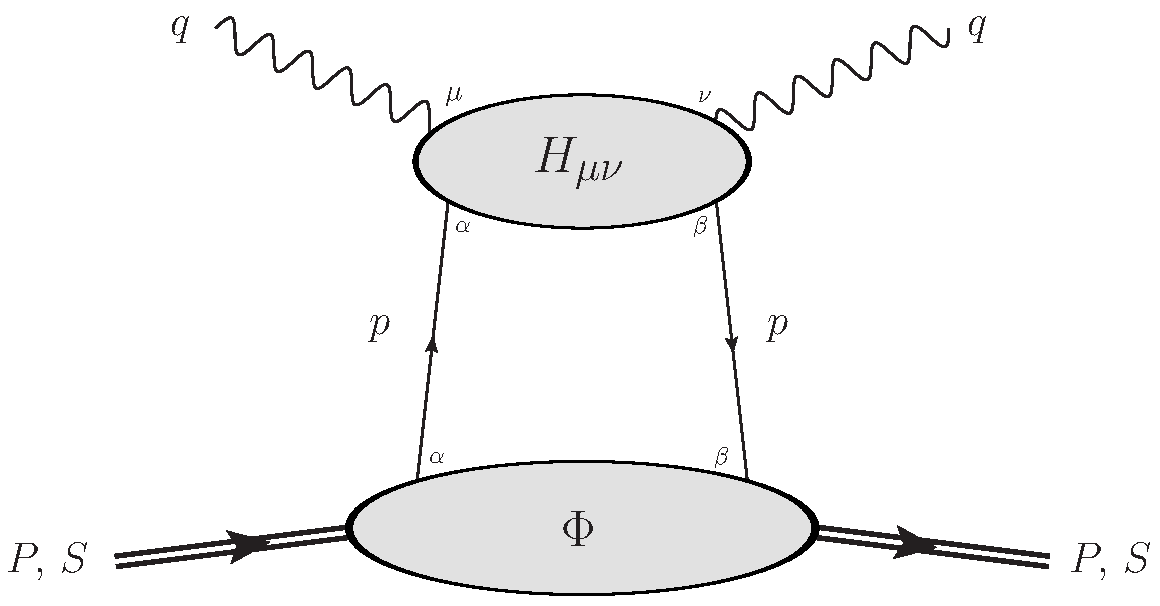
\includegraphics[width=0.5\textwidth]{DIS_FT.pdf} 
  \caption{Handbag diagram for DIS in the field theoretic model.}
  \label{fig:DIS_FT}
\end{figure}
%%

\subsubsection*{Perturbative corrections and the evolution equation}
The inclusion of gluonic corrections to the Born level introduces divergent contributions. These divergent terms arise from the so-called \textit{mass} or \textit{collinear} singularities that occur because of the effective masslessness of the quarks and are removed by the \textit{factorisation} process. The \textit{factorisation theorem} for DIS~\cite{Collins:1989gx} allows for a separation of the interaction into a 'hard' perturbative part $H^{\mu \nu}_{\alpha \beta}$ (the top 'blob') and a 'soft' non-perturbative part $\Phi_{\alpha \beta}$, represented by the "top" and "bottom" blobs of Fig.~\ref{fig:DIS_FT}, respectively. Schematically, the computation of the hard part gives origin to terms of the form $\alpha_{s} \ln Q^2/m_q^2$, which are split as follows
%-------------------------------
\footnote{Here the divergent contribution is given by the mass term inside the logarithm. However, this term arises only when the computation of the hard part is worked out keeping a non-vanishing mass for the quark. Otherwise, the singularity arises as an infrared logarithmic divergence of the type $\alpha_{s} \ln Q^2/\mathcal{K}^2$, where $\mathcal{K}$ is the cut-off in momentum space.}
%-------------------------------
%%
\begin{equation}
  \alpha_{s} \ln \frac{Q^2}{m_q^2} = \alpha_{s} \ln \frac{Q^2}{\mu^2} + \alpha_{s} \ln \frac{\mu^2}{m_{q}} \,.
\end{equation}
%%
The first term on the r.h.s. is absorbed into the hard part, whereas the other one is absorbed into the soft part (\textit{i.e.} the PDF), which in any case has to be parametrized and studied experimentally. This procedure introduces a \textit{factorisation scale} $\mu^2$, that is the scale at which the separation is made. As a consequence, PDFs acquire a dependence on the scale of the process, whereas the remaining finite part incorporates $Q^2$-dependent terms which correct the expression for the structure functions, thus breaking Bjorken scaling.%

If all orders in perturbation theory were considered, the physical observables would not depend on this scale, thus making the choice of its value completely arbitrary. However, it turns out that predictions are truncated at some fixed order in perturbation theory, and the choice of the values does make some difference. Usually, the optimal choice is $\mu^2 = Q^2$, so that the PDFs will now depend on $x$ and $Q^2$
%%
\begin{equation}
  \Delta f(x)  \hspace{2mm} \longrightarrow \hspace{2mm} \Delta f(x,Q^2) \,.
  \label{eq:Q2_pdf}
\end{equation}
%%
If one keeps only the leading logarithmic (LL) terms proportional to $\alpha_{s} \ln Q^2/\mu^2$, one recovers the PM expressions for the polarised structure functions, Eq.~\eqref{eq:g1_PM}, provided the replacement reported in \eqref{eq:Q2_pdf}.\par
The variation with $Q^2$ is controlled by the Dokshitzer, Gribov, Lipatov, Altarelli and Parisi (DGLAP) evolution equations \cite{Altarelli:1977zs, Dokshitzer:1977sg, Gribov:1972ri}, a set of $(2 n_f + 1)$ coupled integro-differential equations. For the polarised densities, these equations read
%%
%\begin{equation}
%  \begin{split}
%    \frac{\partial}{\partial \ln Q^2} \Delta q_{i} (x,Q^2) = \frac{\alpha_{s}(Q^2)}{4 \pi} \int_{x}^{1} \frac{dy}{y} &\left\{\sum_{k}^{n_f} \left[ \Delta P_{q_i q_k} \left( \frac{x}{y} \right) \Delta q_k(y,Q^2) + \Delta P_{q_i \bar{q}_k} \left(\frac{x}{y}\right) \Delta \bar{q}_k(y,Q^2) \right]\right. \\
%    & \left. + \Delta P_{q_i g} \left(\frac{x}{y}\right) \Delta g (y, Q^2) \right\}
%  \end{split}
%\end{equation}
%%
%\begin{equation}
%  \begin{split}
%    \frac{\partial}{\partial \ln Q^2} \Delta g_{i} (x,Q^2) = \frac{\alpha_{s}(Q^2)}{4 \pi} \int_{x}^{1} \frac{dy}{y} &\left\{\sum_{k=1}^{n_f} \left[ \Delta P_{g q_k} \left( \frac{x}{y} \right) \Delta q_k(y,Q^2) + \Delta P_{g \bar{q}_k} \left(\frac{x}{y}\right) \Delta \bar{q}_k(y,Q^2) \right]\right. \\
%    & \left. + \Delta P_{g g} \left(\frac{x}{y}\right) \Delta g (y, Q^2) \right\}
%  \end{split}
%\end{equation}
%%
\begin{equation}
  \frac{\partial}{\partial \ln Q^2} 
  \left(\begin{matrix}
    \Delta q_i \\
    \Delta g \\
    \Delta \bar{q}_i
  \end{matrix} \right) (x,Q^2) = \frac{\alpha_{s}(Q^2)}{4 \pi}  \sum_{k,l}
  \left(\begin{matrix}
    \Delta P_{q_i q_k} && \Delta P_{q_i g} && \Delta P_{q_i \bar{q}_l} \\
    \Delta P_{g q_k} && \Delta P_{g g} && \Delta P_{g \bar{q}_l} \\
    \Delta P_{\bar{q}_i q_k} && \Delta P_{\bar{q}_i g} && \Delta P_{\bar{q}_i \bar{q}_l} \\
  \end{matrix}\right) \otimes 
  \left(\begin{matrix}
    \Delta q_i \\
    \Delta g \\
    \Delta \bar{q}_i
  \end{matrix} \right) (x,Q^2) \,,
  \label{eq:DGLAP_coupled}
\end{equation}
%%
where $k,l$ run over the quark flavours ($k,l = u,\, d\, s,\, \dots$) and $\otimes$ is the shorthand notation for the convolution product with respect to x
%%
\begin{equation}
  f \otimes g = \int_{x}^{1} \frac{dy}{y} f \left(\frac{x}{y} \right) g(y) \,.
  \label{eq:def_conv}
\end{equation}
%%
The $\Delta P$ are the polarised \textit{splitting functions} and can be expanded in powers of the strong coupling $\alpha_s$
%%
\begin{equation}
  \Delta P = \sum_{n=0}^{\infty} \left( \frac{\alpha_s}{4\pi} \right)^{n} \Delta P^{(n)}(x)\,.
\end{equation}
%%
The evolution equations can be maximally decoupled from each other if one exploits charge conjugation invariance and $SU(n_f)$ flavour symmetry, which impose 
%%
\begin{equation}
  \begin{split}
    & \Delta P_{q_i q_j} = \Delta P_{\bar{q}_i \bar{q}_j} = \delta_{ij} P_{qq}^{V} + P_{qq}^{S} \,,\\
    & \Delta P_{\bar{q}_i q_j} = \Delta P_{q_i \bar{q}_j} = \delta_{ij} P_{\bar{q}q}^{V} + P_{\bar{q}q}^{S} \,,\\
    & \Delta P_{q_i g} = \Delta P_{\bar{q}_i g} = \Delta P_{qg} \,, \\
    & \Delta P_{g q_i} = \Delta P_{g \bar{q}_i} = \Delta P_{gq}
  \end{split}
\end{equation}
%%
Inserting these relations into Eq.~\eqref{eq:DGLAP_coupled} and using $\Delta q_{i}^{\pm} = \Delta q_{i} \pm \Delta \bar{q}_{i}$,
the evolution equations read 
%%
\begin{equation}
  \begin{split}
    \frac{\partial}{\partial \ln Q^2} 
    \left(\begin{matrix}
      \Delta q_i^{+} \\
      \Delta g \\
      \Delta \bar{q}_i^{-}
    \end{matrix} \right) & = \frac{\alpha_{s}(Q^2)}{4 \pi} 
    \left(\begin{matrix}
      (\Delta P_{qq}^{V} + \Delta P_{q\bar{q}}^{V}) && 2 \Delta P_{qg} && 0 \\
      \Delta P_{gq} && \Delta P_{gg} && 0 \\
      0 && 0 && (\Delta P_{qq}^{V} - \Delta P_{q\bar{q}}^{V})
    \end{matrix} \right) \otimes
    \left(\begin{matrix}
      \Delta q_i^{+} \\
      \Delta g \\
      \Delta \bar{q}_i^{-}
    \end{matrix} \right) 
    \\[10pt]
    & + \frac{\alpha_{s}(Q^2)}{4 \pi}
    \left(\begin{matrix}
      (\Delta P_{qq}^{S} + \Delta P_{q \bar{q}}^{S}) && 0 && 0 \\
      0 && 0 && 0 \\
      0 && 0 && (\Delta P_{qq}^{S} - \Delta P_{q\bar{q}}^{S})
    \end{matrix} \right) 
    \otimes
    \left(\begin{matrix}
      \sum_{k} \Delta q_k^{+} \\
      \Delta g \\
      \sum_{k} \Delta \bar{q}_k^{-}
    \end{matrix} \right)
  \end{split}
\end{equation}
%%
where the dependence on the kinematic has been momentarily omitted. Now the equations are semi-diagonalised, being the third equation completely decoupled from the rest of the system. It is convenient to express the system using the following definitions
%%
\begin{equation}
  \begin{split}
     \Delta \Sigma \equiv \sum_{k=1}^{n_{f}} \Delta q_{k}^{+}  \hspace{10mm} & \T{singlet distribution}\, ,\\
     \Delta V \equiv \sum_{k=1}^{n_{f}} \Delta q_{k}^{-}  \hspace{10mm} & \T{valence distribution}\,, \\
     \Delta q_{NS,is}^{\pm} \equiv \Delta q_{i}^{\pm} - \Delta q_{j}^{\pm} \hspace{10mm} & \T{non-singlet distribution} \,,
  \end{split}
  \label{eq:evb_dist}
\end{equation}
%%
for the polarised parton distributions and
%%
\begin{equation}
  \begin{split}
    & \Delta P^{\pm} \equiv \Delta P_{qq}^{V} \pm \Delta P_{q \bar{q}}^{V} \,,\\
    & \Delta P_{qq} \equiv \Delta P^{+} + n_{f} (\Delta P_{qq}^{S} + \Delta P_{q\bar{q}}^{S} )  \,,\\
    & \Delta P^{V} \equiv \Delta P^{-} + n_{f} (\Delta P_{qq}^{S} - \Delta P_{q \bar{q}}^{S}) \,,
  \end{split}
\end{equation}
%%
for the polarised splitting functions. Hence, the evolution equation can be expressed as follows
%%
\begin{equation}
  \begin{split}
    & \frac{\partial}{\partial Q^2} \Delta g  = \frac{\alpha_{s}(Q^2)}{4 \pi} \Bigl[ \Delta P_{gg} \otimes g + \Delta P_{gq} \otimes \Delta \Sigma \Bigr] \,,\\
    & \frac{\partial}{\partial Q^2} \Delta q^{+}_{i} = \frac{\alpha_{s}(Q^2)}{4 \pi} \Bigl[ \Delta P^{+} \otimes \Delta q_{i}^{+} + \frac{1}{n_f} (\Delta P_{qq} - \Delta P^{+}) \otimes \Delta \Sigma + 2 \Delta P_{qg} \otimes \Delta g \Bigr] \,,\\
    & \frac{\partial}{\partial Q^2} \Delta q^{-}_{i} = \frac{\alpha_{s}(Q^2)}{4 \pi} \Bigl[ \Delta P^{-} \otimes \Delta q_{i}^{-} + \frac{1}{n_f} (\Delta P^{V} - \Delta P^{-}) \otimes \Delta V \Bigr] \,,\\
  \end{split}
  \label{eq:evb_1}
\end{equation}
%%
At this point, it is customary to define the so-called \textit{evolution basis}, a specific set of linear combinations of distributions that maximally decouple the evolution equations. In particular, by looking at the Eqs.~\eqref{eq:evb_1} and using the definitions in Eqs.~\eqref{eq:evb_dist}, it is straightforward to verify that the evolution equations completely decouple for the non-singlet and valence distributions
%%
\begin{equation}
  \begin{split}
    & \frac{\partial}{\partial \ln Q^2}\Delta q_{\T{NS}ij}^{\pm} (x,Q^2) = \frac{\alpha_s(Q^2)}{4\pi} \Delta P^{\pm} \otimes \Delta q_{{\T{NS}ij}}^{\pm} (x,Q^2) \,, \\
    & \frac{\partial}{\partial \ln Q^2}\Delta V (x,Q^2) = \frac{\alpha_s(Q^2)}{4\pi} \Delta P^{V} \otimes \Delta V (x,Q^2)\,,
  \end{split}
\end{equation}
%% 
whereas the singlet and the gluon distributions remain coupled 
%%
\begin{equation}
  \frac{\partial}{\partial \ln Q^2} 
  \left(\begin{matrix}
    \Delta g (x,Q^2)\\
    \Delta \Sigma (x,Q^2)
  \end{matrix} \right) 
  = \frac{\alpha_{s}(Q^2)}{4 \pi} \otimes
  \left(\begin{matrix}
    \Delta P_{gg} && \Delta P_{gq} \\
    \Delta P_{qq} && \Delta 2n_f P_{qg}
  \end{matrix} \right)
  \otimes 
  \left(\begin{matrix}
    \Delta g (x,Q^2) \\
    \Delta \Sigma (x,Q^2)
  \end{matrix} \right) \,.
\end{equation}
%%
The dependence on the kinematics $(x,Q^2)$ have been restored.%

The polarised splitting functions have been computed at LO in Ref.~\cite{Altarelli:1977zs}, then extended at NLO in Ref.~\cite{Mertig:1995ny, Vogelsang:1995vh}; only recently splitting functions have been computed at NNLO in Ref.~\cite{Moch:2014sna}.%

Finally, a little complementary observation about the factorisation theorem. In principle, there could be several contributions to the process in the field theoretic approach. The factorisation theorem only refers to Fig.~\ref{fig:DIS_FT}, which represents the leading region for DIS when the light-cone gauge, $A^{+}=0$, is adopted. All the contributions coming from this diagram are called 'leading twist'. All the diagrams other than that shown in Fig.~\ref{fig:DIS_FT} have an overall suppression of order $(1/Q)^{n}$ and provide the so-called 'higher twist' corrections. Therefore, the complete expression for observables like structure functions should read
%%
\begin{equation}
  F(x, Q^2) = F(x, Q^2)^{LT} + \frac{F^{(1)}(x,Q^2)}{Q^2} + \dots \,.
\end{equation}
%%
There are two types of twist corrections -- target mass corrections, which are purely kinematical, and dynamical corrections. Regardless the origin of these contributions, they can be neglected by means of kinematic cuts applied to the data set, so that the small-$Q^2$ region is excluded. Kinematic cuts will be further discussed in Chap.~\ref{ch:4}, where the data sets will be presented.

\subsubsection*{The gluon contribution to $g_1$}
Another important consequence of the QCD analysis is the rise of the contribution from polarised gluons to the structure function $g_1$. Indeed, the leading-twist expression becomes 
%%
\begin{equation}
  g_1(x,Q^2) = \frac{1}{2} \sum_{i=1}^{n_f} e_{q}^2 \Biggl\{ \Delta \mathcal{C}_{q} \otimes \Bigl[ \Delta q_i (x,Q^2) + \Delta \bar{q}_i (x,Q^2) \Bigr] + \Delta \mathcal{C}_{g} \otimes \Delta g (x,Q^2)\Biggr\} \,,
  \label{eq:g1_QFT}
\end{equation}
%%
where the gluon contribution is defined as
%%
\begin{equation}
  \Delta g(x,Q^2) = g^{\uparrow}(x,Q^2) - g^{\downarrow}(x,Q^2) \,.
\end{equation}
%%
In Eq.~\eqref{eq:g1_QFT}, the sum runs over the flavours of quarks and antiquarks, $\otimes$ denotes the usual convolution in Eq.~\eqref{eq:def_conv}, and finally $\Delta \mathcal{C}_{q}$ and $\Delta \mathcal{C}_{g}$ are the \textit{coefficient functions} which are related to the hard photon-quark or photon-gluon cross-sections. Coefficient functions are perturbative quantities and can be expanded in a power series of $\alpha_s$
%%
\begin{equation}
  \Delta \mathcal{C} \left( y, \alpha_s \right) = \Delta \mathcal{C}^{(0)}_{p} (y) + \frac{\alpha_s}{4\pi} \Delta \mathcal{C}^{(1)}_{p} (y) + \mathcal{O}(\alpha_s^2)\,,
\end{equation}
%% 
where $p=q,g$ and
%%
\begin{equation}
  \left\{ \hspace{-3mm}
  \begin{array}{cl}
    &\Delta \mathcal{C}_{q}^{(0)} (y) = \delta(1-y)\,,\\[10pt]
    &\Delta \mathcal{C}_{g}^{(0)} (y) = 0 \,.\\
  \end{array}
  \right.
\end{equation}
%%
At the lowest order, the gluon distribution does not contribute to the structure function, hence the Naive Parton Model expectation, Eq.~\eqref{eq:g1_PM}, is recovered. At higher orders, the simple and intuitive picture provided by the PM no longer holds, and the Bjorken variable $x$ loses its interpretation as fractional momentum.\par
Now that I have introduced the polarised gluon distribution, it is possible to revise the unexpected result, Eq.~\eqref{eq:EMC_exp}. In the PM, the axial current $a_0$ can be regarded as the spin quark operator, since it is related to the first moment of the singlet quark distribution. The key point is that the axial current $a_0$ is conserved only in a massless and \textit{free-field} theory. However, when one allows for interactions among quarks, the current is no longer conserved, even when the masses of partons are neglected. In principle, one should not be worried about that, given that the conserved quantity is the total angular momentum $J_z$ and not $S_z$, so that the physical interpretation of $a_0$ as the spin operator of quark remains valid. However, it turns out that the current is not conserved because of an anomalous contribution coming from the triangle diagram that arises from the axial gluon current. This suggests that an additional contribution to the proton spin has not been considered in the expectation value of the axial current in the PM.%

It can be shown (see \textit{e.g.} Ref.~\cite{Anselmino:1993tc}) that the gluon contribution to the structure function $g_1$ modifies the expectation value of the singlet axial current by a term that reads
%%
\begin{equation}
  a_{0}^{\T{gluons}}(Q^2) = - n_{f} \frac{\alpha_s(Q^2)}{2\pi} \int_{0}^{1} dx \, \Delta g (x, Q^2) \,,
\end{equation}
%%
where $n_{f}$ indicates the number of active flavours that effectively participate in the analysis (in this case, $n_f = 3$ since we are considering only the lightest quarks $u,d$ and $s$). In the literature, this term is regarded as the gluon anomaly, and the expectation of the axial current $a_0$ should read
%%
\begin{equation}
  a_{0} (Q^2) = \Delta \Sigma (Q^2) - 3 \frac{\alpha_{s}(Q^2)}{2\pi} \Delta g (Q^2) \,,
  \label{eq:a0_gluon}
\end{equation}
%%
where I have considered $n_f = 3$ active flavours. Here, $\Delta \Sigma(Q^2)$, $\Delta g(Q^2)$ represent the first moment of the singlet and gluon distributions, respectively. What the EMC experiment actually measured was the total singlet axial charge $a_0$. The l.h.s. of this expression has the fundamental implication that the small measured value of $a_0$ can now be explained as a cancellation between the two terms, reconciling the discrepancy between the EMC result and the theoretical expectation.\par Now, as a general rule, the PM can be derived from perturbative QCD in the limit $Q^2 \rightarrow \infty$, since the running coupling $\alpha_s$ vanishes and the free-theory is recovered. However, an exception to this rule is the gluon contribution in Eq.~\eqref{eq:a0_gluon}. Even though $a_{0}^{\T{gluons}}$ may be seen as a perturbative correction to $a_0$, the gluon contribution does not decouple in the limit $Q \rightarrow \infty$. Indeed, it can be shown either from the spin-dependent DGLAP evolution equations~\cite{Borah:2012ey} or from the anomalous dimensions of the operators involved~\cite{Anselmino:1994gn}, that the logarithmic decrease of $\alpha_s$ as $Q^2 \rightarrow \infty$ is compensated by the increase in the gluon helicity distribution. This is a direct consequence of the contribution induced by the axial anomaly in the triangle diagram. Furthermore, the initial physical interpretation of $\Delta \Sigma (Q^2)$ relied on the conservation of the singlet axial current $a_0$. There is no reason for the first moment of the singlet distribution to coincide with the value of the constituent quark model once the current is not conserved. This inconsistency is also made clearer by the fact that the first moment of the singlet distribution, being related to a not conserved quantity, acquires a scale dependence, that reifies in a $Q^2$ dependence. It is then clear that an observable quantity, such as the spin of the quarks, cannot depend on an in-principle arbitrary quantity such as the scale, making the physical significance of the singlet quark distribution $\Delta \Sigma(x,Q^2)$ a matter of a careful definition, as I will explain later.%

Finally, it is possible to give a rough estimate of the gluon helicity. The expected spin contribution carried by quarks is $\Delta \Sigma \simeq (0.6  \div 0.7)$. To accomplish the huge cancellation enclosed in the singlet axial charge, the gluon contribution at $Q^2 \simeq 10 \, \T{GeV}^2$ should be $\Delta g \simeq 4$. Despite the large value, it cannot be ruled out in that the QCD evolution equations increase indefinitely the value of $\Delta g$ with $Q^2$. Furthermore, angular momenta must satisfy a helicity sum rule which generally reads
%%
\begin{equation}
  J_{z} = S_{z}^{q} + S_{z}^{g} + L_z = \frac{1}{2} \,, 
  \label{eq:J_z_sumrule}
\end{equation} 
%%
where $L_z$ represents the total angular momentum of all partons. Hence, in order for Eq.~\eqref{eq:J_z_sumrule} to be fulfilled, the growing value of $S_{z}^{g}$ has to be compensated by an analogous growth in the magnitude of $L_{z}$. Since a measurement of the orbital momentum of partons is hardly achievable, the only possibility to estimate this contribution is by determining both quarks and gluon contributions from experimental data, providing a reliable accuracy.
%The goal of this thesis is to provide such estimates, by scrutinizing both the available experimental data and the methodology.

\subsection{Scheme dependence}
The divergent contributions coming from higher order corrections are regulated by normalisation, which introduces a dependence on the chosen scheme. Despite the fact that the choice is completely arbitrary, it may strongly affect the results and compromise the physical interpretation of certain quantities, as I showed in the section before. Here, I just outline the direct consequences of different schemes, without providing any details. A pedagogical introduction to the scheme dependence may be found in Ref.~\cite{leader_2001} and reference therein. 
\begin{enumerate}
  \item The most frequently used renormalization scheme is the $\overline{\T{MS}}$-scheme, in which the gluon coefficient functions vanish. As a result, there is no gluon contribution to the first moment of the structure function $g_1$. The first moment of the singlet quark distribution, $\Delta \Sigma (Q^2)$, varies with $Q^2$ and any interpretation as the total spin carried by quarks no longer holds. Hence, the singlet axial charge 
  %%
  \begin{equation}
    a_0 (Q^2) = \int_{0}^{1} dx \,  \left.\Delta \Sigma(x,Q^2) \right|_{\overline{\T{MS}}} \,,
    \label{eq:MSB_scheme}
  \end{equation}
  %%
  cannot be compared with the constituent quark result. Finally, the first moment of the non-singlet triplet and octet distributions,
  %%
  \begin{equation}
    a_3 = \int_{0}^{1} dx \, \Delta T_3 (x,Q^2) \,, \hspace{10mm} a_8 = \int_{0}^{1} dx \, \Delta T_8 (x,Q^2) \,,
    \label{eq:a3_a8}
  \end{equation}
  %% 
  do not have any $Q^2$-dependence. Eqs.~\eqref{eq:a3_a8} will be adopted as theoretical assumptions in order to further constraint the PDF determination, as discussed in the next chapter.
  
  \item The other renormalization scheme is due to Adler and Bardeen (AB), and is defined such that the first moment of the singlet distribution is independent of $Q^2$, restoring the physical interpretation as the total spin carried by quarks. The gluon distribution is the same as in the $\overline{\T{MS}}$-scheme, but now it contributes to the first moment of the gluon of the structure function $g_1$
  %%
  \begin{equation}
    a_{0}(Q^2) = \int_{0}^{1} dx \, \left. \Delta \Sigma (x,Q^2) \right|_{\T{AB}} - n_f \frac{\alpha_s(Q^2)}{2\pi} \int_{0}^{1} dx \, \Delta g(x,Q^2) \,.
    \label{eq:AB_scheme}
  \end{equation}
\end{enumerate}
The two approaches are related by comparing Eq.~\eqref{eq:MSB_scheme} with Eq.~\eqref{eq:AB_scheme}
%%
\begin{equation}
  \int_{0}^{1} dx \, \left. \Delta \Sigma (x,Q^2) \right|_{\T{AB}} = \int_{0}^{1} dx \, \left. \Delta \Sigma (x,Q^2) \right|_{\overline{\T{MS}}} + n_f \frac{\alpha_s(Q^2)}{2\pi}  \int_0^1 dx \, \Delta g(x,Q^2)\,,
  \label{eq:AB-MS}
\end{equation}
%%
It must be noted that the scheme dependence, which highly affects the definition of $\Delta \Sigma (x,Q^2)$, persists even in the limit $Q^2 \rightarrow \infty$. In fact, the two definitions that appear in Eq.~\eqref{eq:AB-MS} differ by a term which is not asymptotically suppressed in this limit, as discussed above. Hence, the definition of the singlet quark first moment is maximally ambiguous.

\section{Semi-inclusive polarised DIS}
\label{sec:SIDIS}

In inclusive DIS, only a limited combination of distributions, Eq.~\eqref{eq:g1_NPM_ev}, is probed by data. In order to achieve a full flavour separation, it is necessary to include information from semi-inclusive processes. In particular, I will consider data from semi-inclusive deeply inelastic processes, which are the same as inclusive DIS, except that a certain hadron (typically a pion or a kaon) is detected in the final state. The process may be sketched as
%%
\begin{equation}
  \ell + N \longrightarrow \ell' + h +  X \,,
    \label{eq:SIDIS}
\end{equation}
%%
where $h$ represents the detected hadron. As with DIS, the squared amplitude factorises into a leptonic and a hadronic part. While the former does not get modified, the latter now reads \cite{collins_2011}
%%
\begin{equation}
  W^{\mu \nu} (q,P) = \frac{1}{4\pi} \sumint_{X} d^4 z \, e^{i q \cdot z} \, \bra{0} j^{\mu}(z/2) \ket{P,X,\T{out}} \, \bra{P,X,\T{out}} j^{\nu}(-z/2) \ket{0}\,.
\end{equation}
%%
Because a particular hadron is detected in the final state, it is not possible to eliminate the sum $\sumint_{X}$. This dependence on the final state hadron reifies in the introduction of an additional non-perturbative quantity - the fragmentation function (FF). A detailed analysis on this new soft contribution is beyond the scope of this Thesis, and I refer to Ref.~\cite{Metz:2016swz} for a formal introduction to FFs. For the present work, it is necessary to note that FFs provide the analogue for PDFs for the final hadronization state, that is how quarks and gluons combine into a colour-neutral particle such as hadrons. The FF is denoted by $D^{h/i}(z)$ and describes the fragmentation of an unpolarised parton of type $i$ into an unpolarised hadron of type $h$. The variable $z$ is the counterpart of the Bjorken variable $x$ and, in the intuitive picture provided by the PM, it represents the fraction of the parton momentum carried by the detected hadron. Again, in the simpified picture of the PM, the momentum fraction $z$ only refers to the longitudinal component along the direction of motion of the parton. In the PM, the quantity $D^{h/i}(z)dz$ can be interpreted as the number of hadrons $h$ originating from the parton $i$ with momentum faction in $[z, z+dz]$, although such a view is modified when accounting for higher-order QCD corrections.%

\begin{figure}[t]
  \centering
  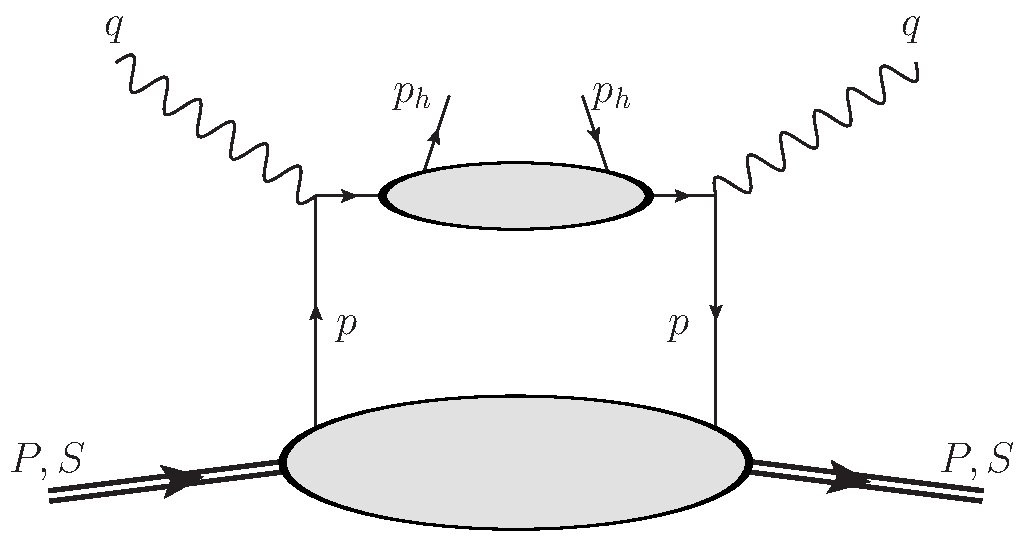
\includegraphics[width=0.5\textwidth]{SIDIS_2.pdf} 
  \caption{Parton model for SIDIS.}
  \label{fig:SIDIS_PM}
\end{figure}

The kinematic variables are the same of DIS, Eqs.~(\ref{eq:nu}-\ref{eq:W2}), with the additional variable
%%
\begin{equation}
  z = \frac{P \cdot p_h}{P \cdot q} \,,
\end{equation}
%%
where $p_h$ is the four-momentum of the detected hadron. The PM approximation of the process is displayed in Fig.~\ref{fig:SIDIS_PM}.\par
For collisions with longitudinally polarised leptons and targets, the polarised structure function can be isolated by taking the difference between the cross-sections with opposite target helicities \cite{Abele:2021nyo}
%%
\begin{equation}
  \frac{d \Delta \sigma^h}{dx \, dy \, dz} \equiv  \frac{1}{2} \left(\frac{d^3\sigma_{h}^{\uparrow \Uparrow}}{dx\,dy\,dz} - \frac{d^3\sigma_{h}^{\uparrow \Downarrow}}{dx\,dy\,dz}\right) = \frac{4\pi \alpha_{em}^2}{Q^2} (2-y) g_{1}^{h} (x,\,z,\,Q^2)\,.
\end{equation}
%%
As for DIS, it can be proved (see \textit{e.g.} Ref.~\cite{collins_2011}) that a factorisation theorem holds also for SIDIS processes. The structure function $g_1^h (x,z,Q^2)$ may be written as
%%
\begin{equation}
  \begin{split}
    g_1^{h} (x,z,Q) & = \frac{1}{2} \sum_{q,\bar{q}} e_{q}^2 \left[ \Delta q(x,Q) \otimes \Delta \mathcal{C}_{qq}^{1} \otimes D_{q}^{h}(z,Q) + \right.\\
    & \left.\Delta q(x,Q) \otimes \Delta \mathcal{C}_{gq}^{1} \otimes D^{h}_{g}(z,Q) + \Delta g(x,Q) \otimes \Delta \mathcal{C}_{qg}^{1} \otimes D^{h}_{q}(z,Q) \right] \,,
    \end{split}
    \label{eq:g1h}
\end{equation}
%%
where I have introduced the double convolution defined as 
%%
\begin{equation}
  f \otimes \Delta \mathcal{C} \otimes h (x,z) = \int \frac{d\xi}{\xi} \int \frac{d \zeta} {\zeta} f \left( \frac{x}{\xi}\right)  \, \Delta \mathcal{C} \left(\xi, \zeta\right) \, h \left( \frac{z}{\zeta} \right) \,.
\end{equation}
%%
In a certain sense, the FF "selects" the single flavour in the initial state. This has important phenomenological consequence in the parton determination, as I will discuss in Chap.~\ref*{ch:3}. Phenomenologically, the quantity that is measured in experiments is a normalised asymmetry, similar to Eq.~\eqref{eq:A1}, and takes the form~\cite{deFlorian:2000bm}
%%
\begin{equation}
  A_1^{h}(x,Q^2) \simeq  \frac{\int_{Z} dz \, g_1^h (x,z,Q^2)}{\int_{Z} dz \, F_1^h (x,z,Q^2)} \,,
\end{equation}
%%
where $Z$ denotes the kinematical region covered by final state hadrons.\par
Polarised coefficient functions have been computed at NLO in Ref.~\cite{deFlorian:1997zj} and up to (approximate) NNLO so far in Ref.~\cite{Abele:2021nyo}.%

Similarly to PDFs, FFs contain a $Q^2$-dependence which arises from the factorisation of the ultraviolet divergences. The perturbative dependence on the scale $Q^2$ is given by the same DGLAP equations, Eqs.~\eqref{eq:DGLAP_coupled}
%%
\begin{equation}
  \frac{\partial}{\partial \mu^2} D_{q_i}^{h} (z,\mu^2) = \frac{\alpha_s(\mu^2)}{2\pi} \sum_{j} \int_{z}^{1} \frac{du}{u} P_{ji}\left( u, \alpha_s(\mu^2) \right) \, D_{q_j}^h \left( \frac{z}{u}, \mu^2 \right) \,.
\end{equation}
%% 
The LO splitting function for FFs have been computed in Ref.~\cite{Owens:1978qz, Uematsu:1978yw, Georgi:1977mg}, and they are equivalent to the LO DGLAP splitting functions for PDFs. Splitting functions have been computed at NLO in~\cite{Curci:1980uw, Furmanski:1980cm}, and at NNLO in~\cite{Mitov:2006ic, Moch:2007tx, Almasy:2011eq}.